\chapter{Diagrama de paquetes}
Para el desarrollo de la aplicación se han hecho uso de un conjunto de archivos, organizados en distintos paquetes, los cuales se 
irán definiendo a continuación.\\

Las clases se agruparán mediante el empleo de paquetes que se organizarán mostrando sus relaciones de importación/exportación en un
diagrama de paquetes. Los diagramas de paquetes se usan para representar relaciones lógicas entre distintos elementos como pueden ser
clases y casos de usos, que mantienen una relación semántica entre ellos. \\

   \section{Identificación de paquetes}
   \begin{figure} [H] \begin{center}
   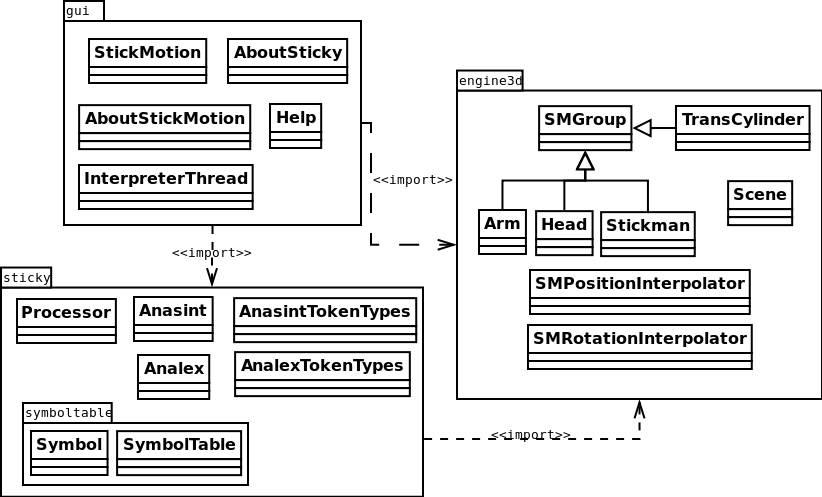
\includegraphics[width=0.7\textwidth]{./imagenes/paquetes}\label{DiagramaPaquetes}
   \caption{Diagrama de paquetes de \textbf{\textit{StickMotion}}.}
   \end{center} \end{figure}
   Se empaquetarán las clases agrupándolas en los siguientes paquetes, correspondiendose con los componentes funcionales en los que se
   descompuso el sistema en el análisis de requisitos. \\

   En la figura \ref{DiagramaPaquetes} se muestra el diagrama indicando las relaciones de importación que se realizan entre los distintos
   paquetes. \\


   \section{Paquete engine3d}
   Este paquete contendrá todo el código relacionado con las animaciones 3D. Incluye las siguientes clases:
   \begin{itemize}
      \item SMGroup.
      \item TransCylinder.java
      \item Arm.java
      \item Head.java
      \item Stickman.java
      \item Scene.java
      \item SMPositionInterpolator.java
      \item SMRotationInterpolator.java
   \end{itemize}


   \section{Paquete gui}
   Este paquete contendrá todo el código relacionado con la interfaz gráfica. Incluye las siguientes clases:
   \begin{itemize}
      \item StickMotion.java
      \item AboutSticky.java
      \item AboutStickMotion.java
      \item Help.java
      \item InterpreterThread.java
   \end{itemize}


   \section{Paquete sticky}
   Este paquete contendrá el código relacionado con ANTLR, y en general, con los tres analizadores. Contiene las siguientes clases:
   \begin{itemize}
      \item Processor.java
      \item analex.g
      \item Analex.java
      \item AnalexTokenTypes.java 
      \item Analex.smap 
      \item AnalexTokenTypes.txt
      \item anasint.g 
      \item Anasint.java 
      \item AnasintTokenTypes.java 
      \item Anasint.smap
      \item AnasintTokenTypes.txt
      \item Asímismo existe también otro paquete, \textbf{\textit{symboltable}}, cuyo contenido es:
            \begin{itemize}
               \item Symbol.java
               \item SymbolTable.java
            \end{itemize}
   \end{itemize}

   Esta maraña de archivos puede verse de manera más clara en la figura \ref{paqueteSymbolTable}.

   \begin{figure} [H] \begin{center}
   \includegraphics[width=0.7\textwidth]{./imagenes/DiagramaPaquetesSymbolTable}\label{paqueteSymbolTable}
   \caption{Diagrama de paquetes para \textbf{\textit{symboltable}}.}
   \end{center} \end{figure}

   A continuación se describen los archivos más importantes de cada uno de los anteriores paquetes.\\

      \subsection{analex.g}
      El analizador léxico es implementado mediante la clase \textbf{\textit{Analex}} que hereda de la clase Lexer. El analizador léxico 
      se encargará del reconocimiento de los tokens y palabras reservadas del lenguaje.\\

      \subsection{anasint.g}
      El analizador sintáctico es implementado por medio de la clase \textbf{\textit{Anasint}}, que hereda de la clase Parser. Esta clase
      se encargará de la definición de las reglas gramaticales del lenguaje.
      

   \section{symboltable}
   Cuando se declara una variable, se crea un objeto del tipo Símbolo que almacena toda la información relacionada con la variable. La 
   información que se almacena de cada variable es la siguientes: 
   \begin{itemize}
      \item Nombre.
      \item Contenido.\\
   \end{itemize}
   Realmente la tabla de símbolos es un array que contiene objetos del tipo Símbolo. Este array contiene todas las variables utilizadas 
   por el lenguaje.\\

   Cada vez que una variable previamente declarada se modifica, la tabla de símbolos es actualizada con el nuevo valor de la variable. No
   importa que cambie el tipo de dato almacenado, ya que el tipado es dinámico y admite cambios en el tipo de la variable en tiempo de ejecución.\\

      \subsection{Symbol.java}
      Este archivo contiene una clase denominada \textbf{\textit{Symbol}}. Esta clase representa a todos y cada uno de los símbolos que  
      componen la tabla de símbolos de nuestro analizador. Es decir por cada variable que se declare en nuestro código, habrá un símbolo
      en nuestra tabla de símbolos. Esta clase también implementa los métodos para la asignación de propiedades al símbolo: nombre y contenido. 

      \subsection{SymbolTable.java}
      Este archivo contiene una clase denominada \textbf{\textit{SymbolTable}}. Esta clase representa la tabla de símbolos de nuestro 
      analizador, que estará compuesta por instancias de la clase Symbol. Esta clase también implementa métodos para la manipulación de
      la tabla, inserción, borrado y búsqueda. 

